\documentclass[10pt]{beamer}

\usetheme[progressbar=frametitle,numbering=fraction]{metropolis}
\usepackage{appendixnumberbeamer}

\usepackage{booktabs}
\usepackage[scale=2]{ccicons}

\usepackage{pgfplots}
\usepgfplotslibrary{dateplot}

\usepackage{xspace}
\newcommand{\themename}{\textbf{\textsc{metropolis}}\xspace}

\usepackage{graphicx}

\title{PhD - a bird's eye view}
\subtitle{Research: doing and writing}
\date{15.05.2018}
\author{Vijay Kartik}
% \institute{Noon Talk, EPFL Library}
% \titlegraphic{\hfill
\includegraphics[height=1cm]{images/epfl_logo.pdf}}

\begin{document}

\maketitle

\begin{frame}{Table of contents}
  \setbeamertemplate{section in toc}[sections numbered]
  \tableofcontents[hideallsubsections]
\end{frame}

\section{My initial dreams}

\begin{frame}{Dreams}
\begin{enumerate}[<+- | alert@+>]
    \item Learn \emph{everything} about (new) PhD topic
    \item Brilliant brainwave
    \item Spread the idea a.k.a Publish articles (maybe 10-20)
    \item BTW, also write some thesis chapters
    \item Applause from everyone
\end{enumerate}
\end{frame}

\begin{frame}{Reality is slightly different}
\begin{enumerate}[<+- | alert@+>]
    \item Learn \emph{some} parts of the PhD topic
    \item Brilliant brainwave
    \item Learn more parts around the PhD topic
    \item Mini-brainwaves - work on them and publish
    \item Go to Step 3
    \item Ah, it's almost 4 years already??
    \item WRITE THE THESIS
    \item Go to step 7
    \item Go to step 7
    \item Applause from parents (probably)
    \item Submit, defend, hunt for jobs
\end{enumerate}

\end{frame}

\section{Useful things I did}

\begin{frame}<1>[label=thingsididlist]{Useful things I did}
    \begin{enumerate}[<+- | alert@+>]
        \item Use a reference manager
        \item Take fairly regular notes of experiments
        \item {Try different collaborative writing tools
        \begin{itemize}
            \item Authorea
            \item Overleaf
            \item PDF + email marathon
            \item Standing over the shoulder and pointing
        \end{itemize}}
        \item Go back and read earlier literature before writing thesis
        \item Automate versioning of all research output
        \item Automate plotting figures [posters, papers, thesis -- everywhere]
        \item Multiple backups of ongoing work
        \item Pre-emptive copyright permissions on own work
    \end{enumerate}
\end{frame}

\begin{frame}{Zotero}
    \includegraphics<1>[width=\columnwidth]{images/zotero}
\end{frame}
\againframe<2>{thingsididlist}

\begin{frame}{Notes}
    \includegraphics<1>[angle=180,width=\columnwidth]{images/log01}
    \includegraphics<2>[angle=180,width=\columnwidth]{images/log02}
\end{frame}
\againframe<3>{thingsididlist}
\againframe<4>{thingsididlist}
\againframe<5>{thingsididlist}
\againframe<6>{thingsididlist}
\againframe<7>{thingsididlist}
\againframe<8>{thingsididlist}
\againframe<9>{thingsididlist}

\begin{frame}{Automate versioning}
    \includegraphics<1>[width=\columnwidth]{images/gitbranch01}
    \includegraphics<2>[width=\columnwidth]{images/gitbranch02}
\end{frame}
\againframe<10>{thingsididlist}

\begin{frame}{Automate plotting}
    \includegraphics<1>[width=0.9\columnwidth]{images/fig02}
    \includegraphics<2>[width=0.9\columnwidth]{images/fig01}
\end{frame}
\againframe<11>{thingsididlist}

\section{More useful things}

\begin{frame}{Useful things I wish I did}
    \begin{enumerate}[<+- | alert@+>]
        \item \emph{Maintain} an organized log (weblog, notebook, tattoos, \emph{anything})
        \item Actively follow up conference discussions
        \item Organize/label data and results better
        \item Write up different research methods tried (and possibly failed)
    \end{enumerate}
\end{frame}

\section{Reusing content in the thesis}

\begin{frame}[fragile]{What content?}
  \begin{description}
  \item[Step 1:] Write a paper
  \item[Step 2:] Done. I now have (unpublished) content.
  \end{description}
  \vspace{1in}
Ideally, I would already start thinking about how much `freedom' I have with \emph{my own} content.
\end{frame}

\subsection{Author's rights}

\begin{frame}[fragile]{(Copy) rights}
  Questions to ask:
  \begin{enumerate}
  \item Can I retain copyright? (Answer: \alert{not always})
  \item Can I provide public access to my paper?
  \item Can I use text/images from my paper in my thesis?
  	\begin{itemize}
  		\item Not to self-plagiarize in another paper!
  	\end{itemize}
  \item Where do I submit?
  \end{enumerate}
  P.S.: Sometimes you do not have a say in which journal to publish in (e.g., supervisor decides for you)
\end{frame}

\begin{frame}{Where do I submit?}
	\begin{figure}
		
\includegraphics[trim={0pt 60pt 0pt 0pt}, clip, width=0.5\columnwidth]{images/xkcdjournal}
	\end{figure}
    \hfill \tiny{Source: https://xkcd.com/1847}
\end{frame}

\begin{frame}{Reusing published content in a presentation}
	\alert{Check first!}
	\begin{figure}
		\frame{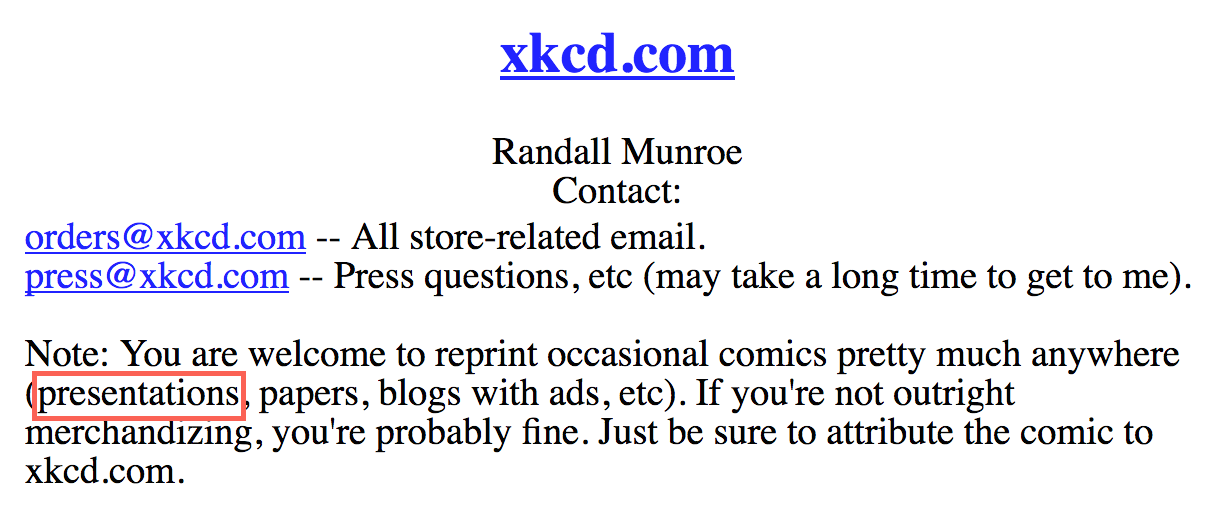
\includegraphics[width=\columnwidth]{images/xkcdpptallowed}}
	\end{figure}
    \hfill \tiny{Source: https://xkcd.com/about}
\end{frame}

\subsection{\mbox{My experience: pre-emptive confirmations}}

\begin{frame}{Advice: Read \emph{before} signing a licence}
\begin{columns}
\hspace{-60pt}
	\begin{column}{0.6\linewidth}
		\begin{figure}
    		\centering
  			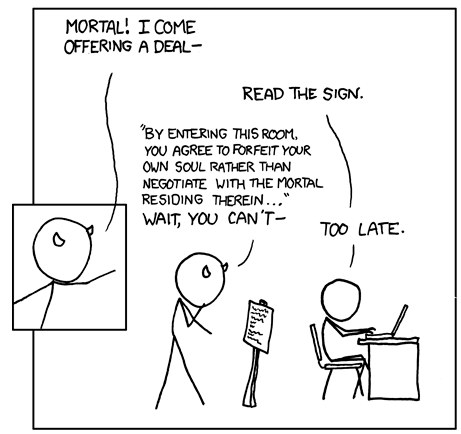
\includegraphics[trim={0pt 0pt 0pt 0pt}, clip, width=\columnwidth]{images/xkcdlicence}
        \end{figure}
        \hfill \tiny{Source: https://xkcd.com/501}
    \end{column}
\hspace{-50pt}
    \begin{column}{0.2\linewidth}
        \begin{figure}
    	    \centering
			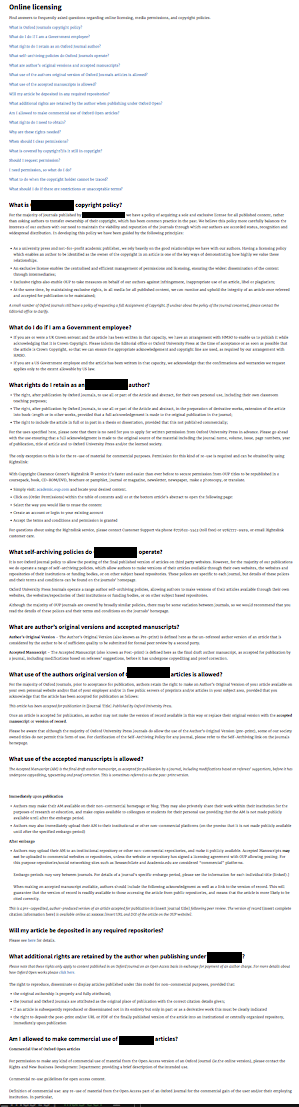
\includegraphics[trim={10pt 0pt 20pt 0pt}, clip, width=\columnwidth]{images/licence}
		\end{figure}
    \end{column}
\end{columns}
\end{frame}

\begin{frame}{Pre/post-prints \& pre/post-embargo}
\begin{columns}
	\begin{column}{0.52\linewidth}
		\begin{figure}
    		\centering
  			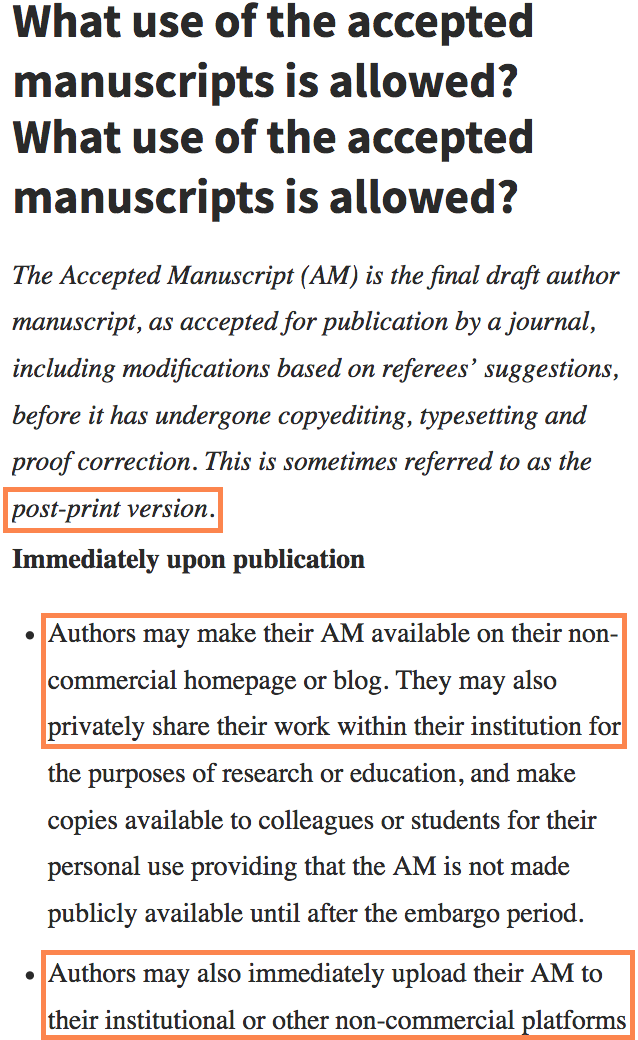
\includegraphics[trim={0pt 0pt 0pt 110pt}, clip, width=\columnwidth]{images/licenceFAQ004a}
        \end{figure}
    \end{column}
    \begin{column}{0.45\linewidth}
        \begin{figure}
    	    \centering
			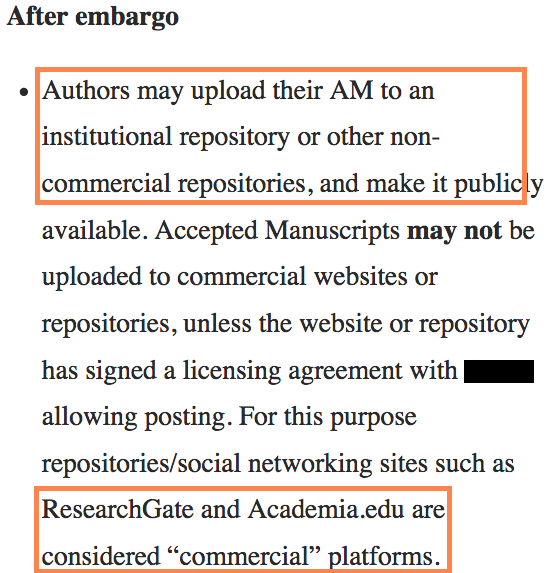
\includegraphics[trim={0pt 0pt 0pt 0pt}, clip, width=\columnwidth]{images/licenceFAQ004b}
		\end{figure}
    \end{column}
\end{columns}
\end{frame}

\begin{frame}{Advice: Look for precise statements}
\hspace{-60pt}
	\begin{figure}
    \centering
		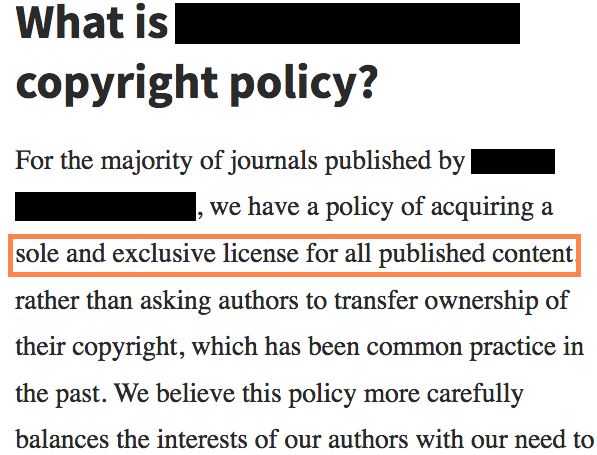
\includegraphics[trim={0pt 0pt 0pt 0pt}, clip, width=\columnwidth]{images/licenceFAQ001}
	\end{figure}
\end{frame}

\begin{frame}{Advice: Check Dos \& Don'ts}
	\begin{figure}
		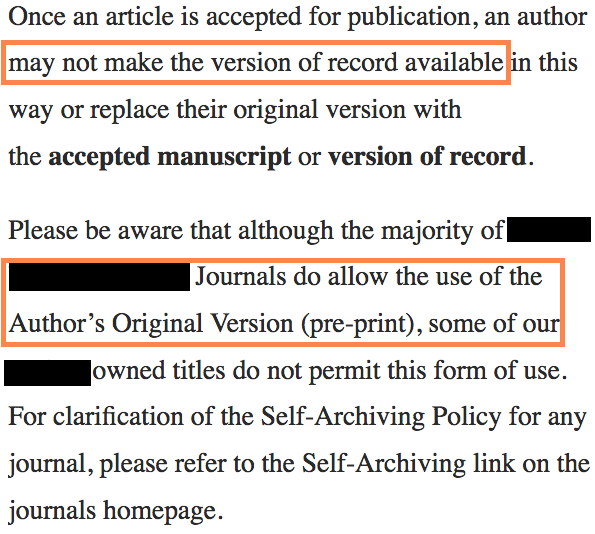
\includegraphics[trim={0pt 30pt 0pt 0pt}, clip, width=\columnwidth]{images/licenceFAQ003}
	\end{figure}
\end{frame}

\begin{frame}{Advice: Ask for \emph{written} clarifications}
	\begin{figure}
		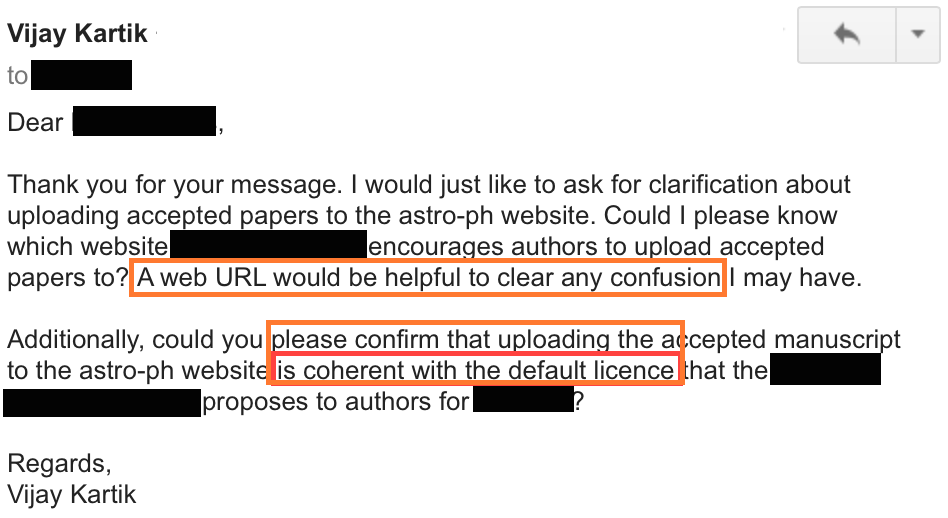
\includegraphics[trim={0pt 0pt 0pt 0pt}, clip, width=0.8\columnwidth]{images/email01}
        
        
\includegraphics[trim={0pt 0pt 0pt 0pt}, clip, width=0.8\columnwidth]{images/email02}
	\end{figure}
\end{frame}

\begin{frame}{Advice: Seek explicit confirmation}
	\begin{figure}
		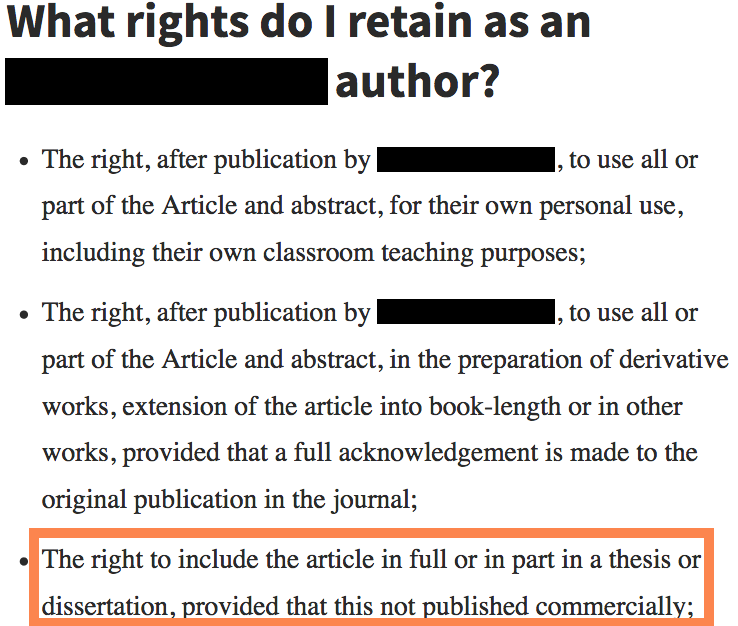
\includegraphics[trim={0pt 0pt 0pt 0pt}, clip, width=0.9\columnwidth]{images/licenceFAQ002}
	\end{figure}
\end{frame}

\section{General research writing tips}

\begin{frame}{General writing tips}
\begin{enumerate}[<+- | alert@+>]
    \item Track progress
    \item Have measurable goals
    \item Get feedback -- often
    \item Defeat writer's block by... writing
    \item Send crap versions to friends/colleagues
    \item Involve your supervisor
    \item Make multiple backups
    \item Convince yourself that the deadline is earlier than it actually is
    \item Get enough sleep
\end{enumerate}
    
\end{frame}

{\setbeamercolor{palette primary}{fg=black, bg=white}
\begin{frame}[standout, plain, noframenumbering]
  Questions?
\end{frame}
}

\begin{frame}[plain, noframenumbering]{Attributions}
  Get the LaTeX source of this presentation from \\
  \textbf{\small{\url{https://github.com/vijaykartik/talk_researchandwriting}}}
  \vspace{0.5in}
  
  The \themename theme used here is made by Matthias Vogelgesang and licensed under a
  \href{http://creativecommons.org/licenses/by-sa/4.0/}{Creative Commons
  Attribution-ShareAlike 4.0 International License}.
  \begin{center}\ccbysa\end{center}
  \vspace{0.5in}
  
  Screenshots of licensing terms FAQs were taken using public access on publishers' online portals.
\end{frame}

\end{document}
